%% Template for MLP Coursework 2 / 22 November 2021 

%% Based on  LaTeX template for ICML 2017 - example_paper.tex at 
%%  https://2017.icml.cc/Conferences/2017/StyleAuthorInstructions

\documentclass{article}
\usepackage[T1]{fontenc}
\usepackage{amssymb,amsmath}
\usepackage{txfonts}
\usepackage{microtype}

% For figures
\usepackage{graphicx}
\usepackage{subcaption} 

% For citations
\usepackage{natbib}

% For algorithms
\usepackage{algorithm}
\usepackage{algorithmic}

% the hyperref package is used to produce hyperlinks in the
% resulting PDF.  If this breaks your system, please commend out the
% following usepackage line and replace \usepackage{mlp2017} with
% \usepackage[nohyperref]{mlp2017} below.
\usepackage{hyperref}
\usepackage{url}
\urlstyle{same}

\usepackage{color}
\usepackage{booktabs} % To thicken table lines
\usepackage{multirow} % Multirow cells in table

% Packages hyperref and algorithmic misbehave sometimes.  We can fix
% this with the following command.
\newcommand{\theHalgorithm}{\arabic{algorithm}}


% Set up MLP coursework style (based on ICML style)
\usepackage{mlp2021}
\mlptitlerunning{MLP Coursework 1 (\studentNumber)}
\bibliographystyle{icml2017}
\usepackage{bm,bbm}


\DeclareMathOperator{\softmax}{softmax}
\DeclareMathOperator{\sigmoid}{sigmoid}
\DeclareMathOperator{\sgn}{sgn}
\DeclareMathOperator{\relu}{relu}
\DeclareMathOperator{\lrelu}{lrelu}
\DeclareMathOperator{\elu}{elu}
\DeclareMathOperator{\selu}{selu}
\DeclareMathOperator{\maxout}{maxout}
\newcommand{\bx}{\bm{x}}




\definecolor{red}{rgb}{0.95,0.4,0.4}
\definecolor{blue}{rgb}{0.4,0.4,0.95}
\definecolor{orange}{rgb}{1, 0.65, 0}

\newcommand{\youranswer}[1]{{\color{red} \bf[#1]}} %your answer: 


%% START of YOUR ANSWERS
%% REPLACE sXXXXXXX with your student number
\def\studentNumber{s2196789}


%% START of YOUR ANSWERS
%% Add answers to the questions below, by replacing the text inside the brackets {} for \youranswer{ "Text to be replaced with your answer." }. 
%
% Do not delete the commands for adding figures and tables. Instead fill in the missing values with your experiment results, and replace the images with your own respective figures.
%
% You can generally delete the placeholder text, such as for example the text "Question Figure 3 - Replace the images ..." 
%
% There are 5 TEXT QUESTIONS. Replace the text inside the brackets of the command \youranswer with your answer to the question.
%
% There are also 3 "questions" to replace some placeholder FIGURES with your own, and 1 "question" asking you to fill in the missing entries in the TABLE provided. 
%
% NOTE! that questions are ordered by the order of appearance of their answers in the text, and not necessarily by the order you should tackle them. You should attempt to fill in the TABLE and FIGURES before discussing the results presented there. 
%
% NOTE! If for some reason you do not manage to produce results for some FIGURES and the TABLE, then you can get partial marks by discussing your expectations of the results in the relevant TEXT QUESTIONS. The TABLE specifically has enough information in it already for you to draw meaningful conclusions.
%
% Please refer to the coursework specification for more details.


%% - - - - - - - - - - - - TEXT QUESTIONS - - - - - - - - - - - - 

%% Question 1:
\newcommand{\questionOne} {
\youranswer{According to Figure 1, the graph of loss and accuracy of VGG 38 experiment is a straight line for both training set and validation set. It represents that the model didn't learn anything after 100 epochs. However, the loss of VGG 08 experiment decreases and the accuracy of that increases as the model is trained in each iteration. By comparing Figure 2 and 3 we could find out what causes this difference. In Figure 2, the gradient flow at each layer remains in a proper range. In Figure 3, the gradient flow at deeper layer is very small, and when it back propagate to shallower layer, the gradient flow is almost 0. Hence we could conclude that the VGG 38 experiment suffers fromt the Vanishing Gradient Problem.  }
}

%% Question 2:
\newcommand{\questionTwo} {
\youranswer{Batch Normalization (BN) uses trainable parameters 
to normalize the input hidden units of each layer. The specific process of how BN works involves with the following equation. Firstly we need to calculate the mean and varaince for a given minibatch:

\begin{equation}
    \label{eq.mean}
    \mu_i \longleftarrow \dfrac{1}{M}\sum_{m=1}^{M}u_i^{m}
\end{equation}

\begin{equation}
    \label{eq.var}
    \sigma_i^2 \longleftarrow  \dfrac{1}{M}\sum_{m=1}^{M}(u_i^m-\mu_i)^2
\end{equation}

After we got the mean and variance for the certain minibatch, we need to this minibatch using the mean and variance we calculated above:

\begin{equation}
    \label{eq.norm}
    \hat{u_i}=\dfrac{u_i-\mu_i}{\sqrt{\sigma_i^2+\epsilon}}
\end{equation}

If we just normalize the bath using the above equation without doing anything else, the neural network won't learn anything from this. The most important thing is that we need to add two learnable parameters $\gamma$ and $\beta$ to scale and shift each instance of the minibatch to make the BN nonlinear.

\begin{equation}
    \label{eq.bn}
    z^i=\gamma_i\hat{u_i}+\beta_i
\end{equation}

At training time we set $\gamma$ and $\beta$ by gradient descent which requires $\gamma$ and $\beta$ differentiable with respect to the loss function. And we will upgrade those values in back propagation using $\dfrac{\partial E}{\partial \hat{u}}$, $\dfrac{\partial E}{\partial \sigma^2}$, $\dfrac{\partial E}{\partial \mu}$ and $\dfrac{\partial E}{\partial u_i}$. At test time the minibatch is normalized at each layer using parameters computed over the complete training data. BN could effectively increase training speed by making the gradient of input of each layer unsaturated and increasing speed of convergence.}
}

%% Question 3:
\newcommand{\questionThree} {
\youranswer{ Residual Connections (RC) is composed of two kind of mapping, identity mapping and residual mapping. In a block of Residual Connection, the identity mapping creates a shortcut connection from the input of a convolutional layer to before the final activation function of that block. The following equation shows what residual learning does in a RC block.

\begin{equation}
    \label{eq.bn}
    y = F(x,{W_i})+x
\end{equation}

The component $x$ is the identity mapping, while $F(x,{W_i})$ is the residual mapping which is the difference between the mapping of convolutional layer and its input $x$. The residual mapping and the identity mapping are added based on element-wise operation . Hence the dimension of their channel must be the same. For different dimension of channels, we could add an additional convectional layer:

\begin{equation}
    \label{eq.bn}
    y = F(x,{W_i})+W_sx
\end{equation}

RC could alleviate the problem of gradient vanishing because it allows the learnt features of shallower layer propagate to deeper layer to get rid of accuracy degradation on deeper layers. During training time the residual mapping is trained until the model is optimal, and the identity mapping ensures the whole neural network being optimal all the time.}
}

%% Question 4:
\newcommand{\questionFour} {
\youranswer{After we implementing both BN and RC to VGG38 model we could find that there is a significant improving on its accuracy and loss. In experiment of BN+RC, we implemented BN on both processing blocks and reduction blocks, and we implemented RC only on processing blocks. By comparing Figure\ref{fig:grad_flow_38} and Figure\ref{fig:grad_flow_bestModel} which shows gradient flow on VGG38 with and without BN+RC, we could find that the gradient flow model implemented with BN and RC is much better and there is no longer gradient vanishing problem anymore. Figure\ref{fig:curves} shows that the accuracy and loss per epoch is much better than the broken neurol network. The accuracy is increasing and the loss is decreasing through each iteration of training.

Moreover, there are some noticeable points according to the experiment results table\ref{tab:CIFAR_results}. Implementing both BN and RC individually on VGG38 model also helps improving its performance, while RC has better performance than BN. On the same learning rate, the combination of BN and RC has the highest training/validation accuracy and the lowest loss, which tells us implementing BN and RC together will give us the best performance. In addition, the model with learning rate of 1e-3 has generally high accuracy than that with learning rate of 1e-2.

By looking at parameters of each model, We could also find that the model implementing with BN has more parameters than that without BN. The difference is because BN adds some additional learnable parameters to normalize the input hidden units of each layer. The more layers in a neural network, the more trainable parameters to be added. We could furthermore run experiments with more layers and number of blocks at each stage and test the performance of BN and RC individually to see how they alleviate the problem of vanishing gradient on deeper neural network comparing with the models on table\ref{tab:CIFAR_results}. We could also implement them on shallower neural network such as VGG08 to see if they helps improving its accuracy or not. Changing the learning rate also affects the performance of model and hence it's worthy to try a different list of learning rate.}
}

%% Question 5:
\newcommand{\questionFive} {
\youranswer{In general, the best model in these combinations of VGG08, VGG38, BN, RC and LR we discussed is VGG38 BN+RC with learning rate of 1e-3. The performance of the model trained could also be improved by adjusting the hyperparmeters of learning rate. Our experiments confirms the effectiveness of BN and RC on resolving problem of gradient vanishing and significant improvement on the accuracy of VGG38 comparing with the broken neural network. From this experiment we evidenced how BN and RC work and the theory behind why they would work. However, we need to do further experiments to test BN and RC on different neural networks with different layers. Whether BN and RC work at the same performance on deeper neural networks still needs to be examined.}
}

%% - - - - - - - - - - - - FIGURES - - - - - - - - - - - - 

%% Question Figure 3:
\newcommand{\questionFigureThree} {
\youranswer{
%
\begin{figure}[t]
    \centering
    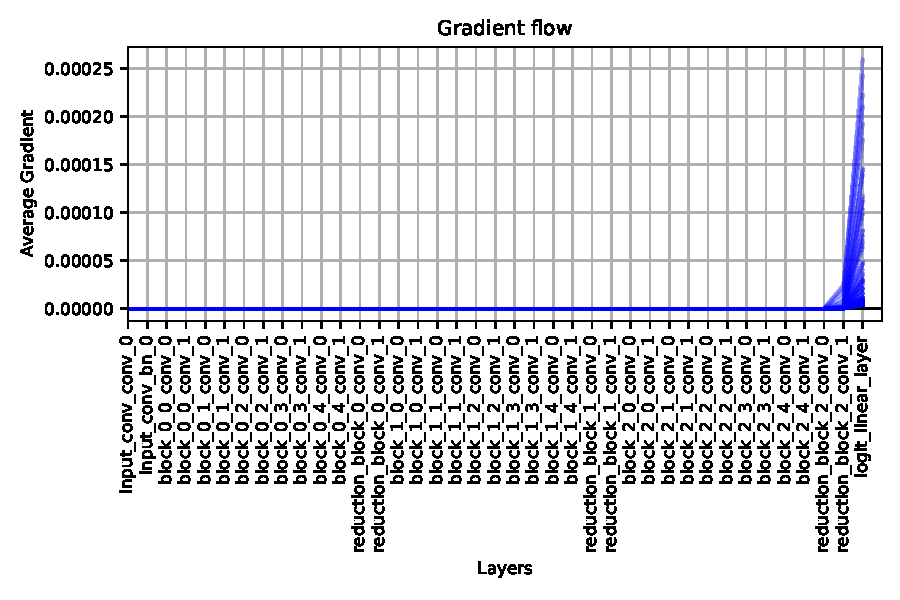
\includegraphics[width=\linewidth]{figures/grad_flow_vgg38.pdf}
    \caption{Gradient Flow on VGG38}
    \label{fig:grad_flow_38}
\end{figure}
}
}

%% Question Figure 4:
\newcommand{\questionFigureFour} {
\youranswer{
%
\begin{figure}[t]
    \begin{subfigure}{\linewidth}
        \centering
        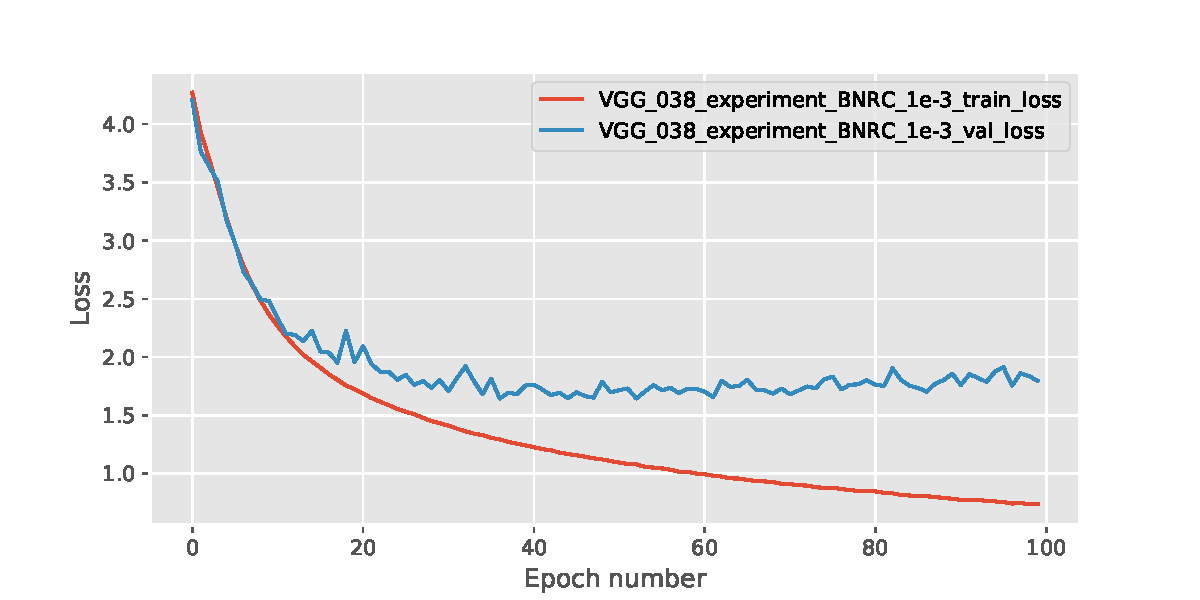
\includegraphics[width=\linewidth]{figures/best_model_loss_performance.pdf}
        \caption{Loss per epoch}
        \label{fig:loss_curves}
    \end{subfigure}

    \begin{subfigure}{\linewidth}
        \centering
        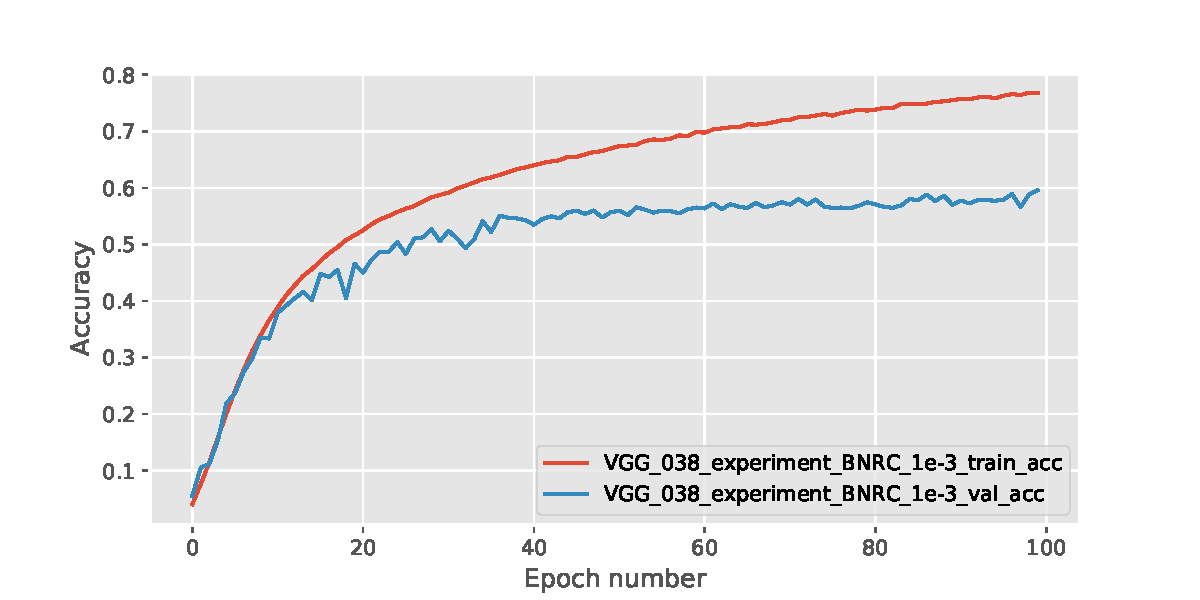
\includegraphics[width=\linewidth]{figures/best_model_accuracy_performance.pdf}
        \caption{Accuracy per epoch}
        \label{fig:acc_curves}
    \end{subfigure}
    \caption{Training curves for VGG38 BN+RC LR1e-3}
    \label{fig:curves}
\end{figure}
}
}

%% Question Figure 5:
\newcommand{\questionFigureFive} {
\youranswer{
%
\begin{figure}[t]
    \centering
    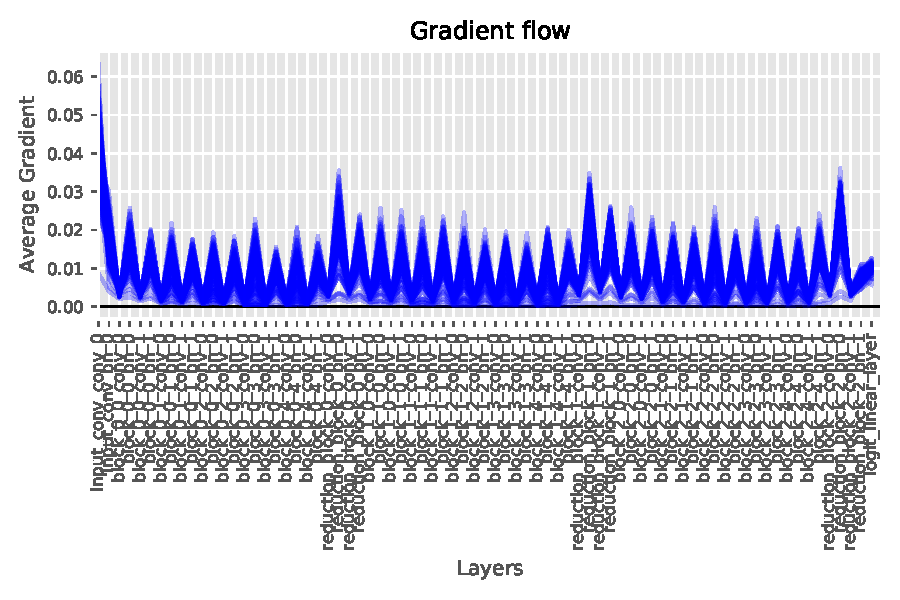
\includegraphics[width=\linewidth]{figures/grad_flow_best.pdf}
    \caption{Gradient Flow on VGG38 BN+RC LR1e-3}
    \label{fig:grad_flow_bestModel}
\end{figure}
}
}

%% - - - - - - - - - - - - TABLES - - - - - - - - - - - - 

%% Question Table 1:
\newcommand{\questionTableOne} {
\youranswer{
%
\begin{table*}[t]
    \centering
    \begin{tabular}{lr|ccccc}
    \toprule
        Model                   & LR   & \# Params & Train loss & Train acc & Val loss & Val acc \\
    \midrule
        VGG08                   & 1e-3 & 60 K    &  1.74      & 51.59     & 1.95     & 46.84 \\
        VGG38                   & 1e-3 & 336 K   &  4.61      & 00.01     & 4.61     & 00.01 \\
        VGG38 BN                & 1e-3 & 339 K   &  1.47      & 57.94     & 1.88     & 48.60 \\
        VGG38 RC                & 1e-3 & 336 K   &  1.33      & 61.52     & 1.84     & 52.32 \\
        VGG38 BN + RC           & 1e-3 & 339 K   &  0.74      & 76.76     & 1.79     & 59.56 \\
        VGG38 BN                & 1e-2 & 339 K   &  1.75      & 50.73     & 2.01     & 45.84 \\
        VGG38 BN + RC           & 1e-2 & 339 K   &  0.72      & 76.86     & 1.86     & 57.60  \\
    \bottomrule
    \end{tabular}
    \caption{Experiment results (number of model parameters, Training and Validation loss and accuracy) for different combinations of VGG08, VGG38, Batch Normalisation (BN), and Residual Connections (RC), LR is learning rate.}
    \label{tab:CIFAR_results}
\end{table*} 
}
}

%% END of YOUR ANSWERS
%% END of YOUR ANSWERS



%% Do not change anything in this file. Add your answers to mlp-cw1-questions.tex



\begin{document} 

\twocolumn[
\mlptitle{MLP Coursework 2}
\centerline{\studentNumber}
\vskip 7mm
]

\begin{abstract} 
Deep neural networks have become the state-of-the-art 
in many standard computer vision problems thanks to more powerful
neural networks and large labeled datasets.
While very deep networks allow for better deciphering
of the complex patterns in the data,
training these models successfully is a challenging task
due to problematic gradient flow through the layers, 
known as vanishing/exploding gradient problem (VGP and EGP respectively).
In this report, we first analyze this problem in VGG models
with 8 and 38 hidden layers on the CIFAR100 image dataset, 
by monitoring the gradient flow during training. 
We explore known solutions to this problem including batch
normalization or residual connections, and explain their theory
and implementation details. 
Our experiments show that batch normalization and residual connections effectively
address the aforementioned problem and hence enable a deeper model to outperform
shallower ones in the same experimental setup.
\end{abstract} 

\section{Introduction}
\label{sec:intro}
Despite the remarkable progress of deep neural networks in image classification problems~\cite{simonyan2014very, he2016deep}, training very deep networks is a challenging procedure.
One of the major problems is the VGP, a phenomenon where gradients from the loss function shrink to zero as they backpropagate
to earlier layers, hence preventing the network from updating its
weights effectively. 
This phenomenon is prevalent and has been extensively
studied in various deep network including feedforward  networks~\cite{glorot2010understanding}, 
RNNs~\cite{bengio1993problem}, and CNNs~\cite{he2016deep}. 
Multiple solutions have been proposed to mitigate this problem by using
weight initialization strategies~\cite{glorot2010understanding},
activation functions~\cite{glorot2010understanding},
input normalization~\cite{bishop1995neural},
batch normalization~\cite{ioffe2015batch}, and shortcut
connections \cite{he2016deep, huang2017densely}.

This report focuses on diagnosing the VGP occurred in the VGG38 model and addressing
it by implementing two standard solutions.
In particular, we first study the ``broken''
network in terms of its gradient flow, norm of gradients with respect to
model weights for each layer and contrast it 
to ones in the healthy VGG08 to pinpoint the problem.
Next, we review two standard solutions for this problem, 
batch normalization (BN)~\cite{ioffe2015batch} and residual connections (RC)~\cite{he2016deep}
in detail and discuss how they can address the gradient problem.
We first incorporate batch normalization (denoted as VGG38+BN), 
residual connections (denoted as VGG38+RC), 
and their combination (denoted as VGG38+BN+RC) to the given VGG38 architecture.
We train the resulting three configurations, and VGG08 and VGG38 models on 
CIFAR-100 dataset and present the results.
The results show that though separate use of BN and RC does tackle 
the vanishing/exploding gradient problem, therefore enabling the training of the VGG38 model, 
the best results are obtained by combining both BN and RC.

%


\section{Identifying training problems of a deep CNN}
\label{sec:task1}

\begin{figure}[t]
    \begin{subfigure}{\linewidth}
        \centering
        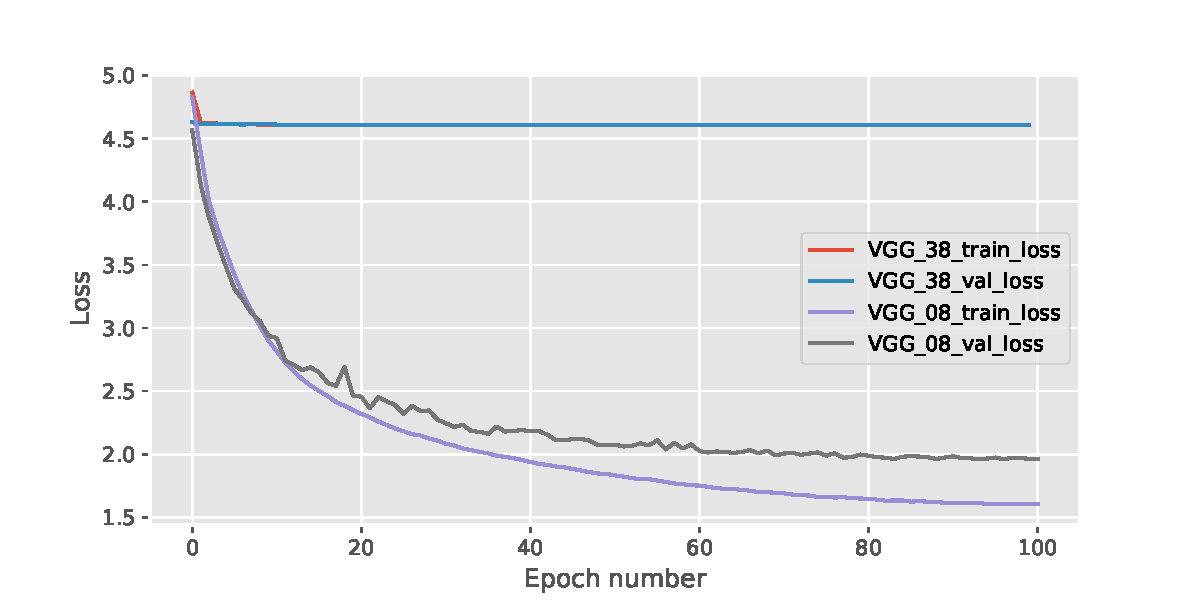
\includegraphics[width=\linewidth]{figures/loss_plot.pdf}
        \caption{Loss per epoch}
        \label{fig:loss_curves}
    \end{subfigure}

    \begin{subfigure}{\linewidth}
        \centering
        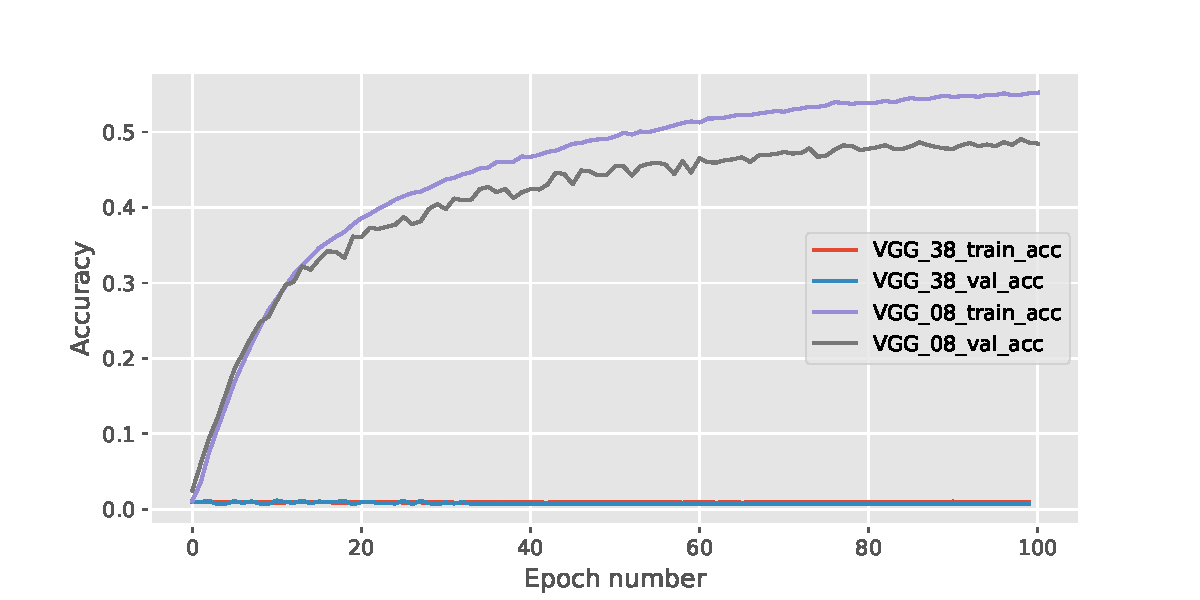
\includegraphics[width=\linewidth]{figures/accuracy_plot.pdf}
        \caption{Accuracy per epoch}
        \label{fig:acc_curves}
    \end{subfigure}
    \caption{Training curves for VGG08 and VGG38}
    \label{fig:curves}
\end{figure}

\begin{figure}[t]
    \centering
    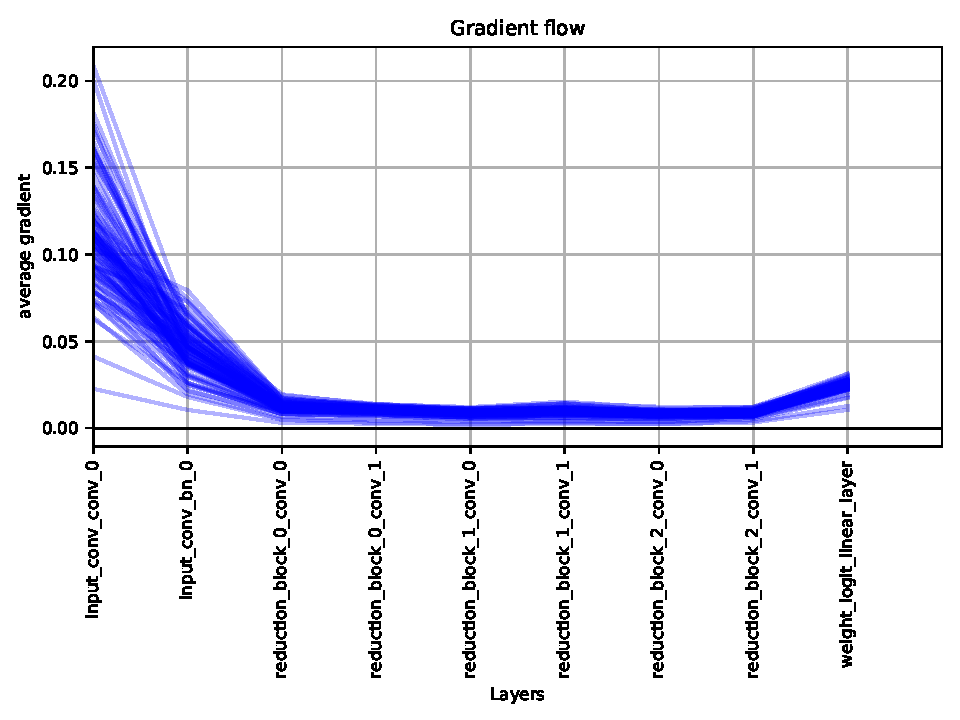
\includegraphics[width=\linewidth]{figures/grad_flow_vgg08.pdf}
    \caption{Gradient flow on VGG08}
    \label{fig:grad_flow_08}
\end{figure}

\questionFigureThree

Concretely, training deep neural typically involves three steps, forward
pass, backward pass (or backpropagation algorithm~\cite{rumelhart1986learning}) and weight update.
The first step involves passing the input $x^0$ to the network and producing 
the network prediction and also the error value.
In detail, each layer takes in the output of the previous layer and applies
a non-linear transformation:
\begin{equation}
\label{eq.fprop}
\bx^{(l)} = f^{(l)}(\bx^{(l-1)}; W^{(l)})    
\end{equation} 
where $(l)$ denotes the $l$-th layer in $L$ layer deep network,
$f^{(l)}(\cdot,W^{(l)})$ is 
a non-linear transformation for layer $l$, and $W^{(l)})$ are the 
weights of layer $l$.
For instance, $f^{(l)}$ is typically a convolution operation followed by an activation
function in convolutional neural networks.
The second step involves the backpropagation algorithm, where we calculate
the gradient of an error function $E$ (e.g. cross-entropy) for each layer's
weight as follows:

\begin{equation}
    \label{eq.bprop}
\frac{\partial E}{\partial W^{(l)}} = \frac{\partial E}{\partial \bx^{(L)}} \frac{\partial \bx^{(L)}}{\partial \bx^{(L-1)}} \dots \frac{\partial \bx^{(l+1)}}{\partial \bx^{(l)}}\frac{\partial \bx^{(l)}}{\partial W^{(l)}}.
\end{equation}

This step includes consecutive tensor multiplications between multiple
partial derivative terms.
The final step involves updating model weights by using the computed 
$\frac{\partial E}{\partial W^{(l)}}$ with an update rule.
The exact update rule depends on the optimizer.

A notorious problem for training deep neural networks is the vanishing/exploding gradient
problem~\cite{bengio1993problem} that typically occurs in the backpropagation step when some of partial gradient terms in Eq.~\ref{eq.bprop} includes values larger or smaller than 1.
In this case, due to the multiple consecutive multiplications, the gradients w.r.t. weights
can get exponentially very small (close to 0) or very large (close to infinity) and
prevent effective learning of network weights.


%


Figures~\ref{fig:grad_flow_08} and \ref{fig:grad_flow_38} depict the gradient flows through
VGG architectures \cite{simonyan2014very} with 8 and 38 layers respectively,
trained and evaluated for a total of 100 epochs on the 
CIFAR100 dataset. \questionOne.


\section{Background Literature}
\label{sec:lit_rev}
In this section we will highlight some of the most influential
papers that have been central to overcoming the VGP in
deep CNNs.

\paragraph{Batch Normalization}\cite{ioffe2015batch}
BN seeks to solve the  problem of 
internal covariate shift (ICS), when distribution of each layer’s 
inputs changes during training, as the parameters of the previous layers change. 
The authors
argue that without batch normalization, the distribution of
each layer’s inputs can vary significantly due to the 
stochastic nature of randomly sampling mini-batches from your
training set. Layers in the network hence must continuously
adapt to these high variance distributions which hinders the
rate of convergence gradient-based optimizers. This optimization
problem is exacerbated further with network depth due
to the updating of parameters at layer $l$ being dependent on
the previous $l-1$ layers.

It is hence beneficial to embed the normalization of
training data into the network architecture after work from
LeCun \emph{et al.} showed that training converges faster with
this addition \cite{lecun2012efficient}. Through standardizing
the inputs to each layer, we take a step towards achieving
the fixed distributions of inputs that remove the ill effects
of ICS. Ioffe and Szegedy demonstrate the effectiveness of
their technique through training an ensemble of BN
networks which achieve an accuracy on the ImageNet classification
task exceeding that of humans in 14 times fewer
training steps than the state-of-the-art of the time.
It should be noted, however, that the exact reason for
BN’s effectiveness is still not completely understood and it is 
an open research question~\cite{santurkar2018does}.



\paragraph{Residual networks (ResNet)}\cite{he2016deep}
One interpretation of how the VGP arises is that stacking non-linear layers
between the input and output of networks makes the
connection between these variables increasingly
complex. This results in the gradients becoming
increasingly scrambled as they are propagated back through
the network and the desired mapping between input and output
being lost. He~\emph{et al.} observed this on 
a deep 56-layer neural network counter-intuitively
achieving a higher training error than a shallower 20-
layer network despite higher theoretical power.
Residual networks, colloquially
known as ResNets, aim to alleviate this through the
incorporation of skip connections that bypass the linear
transformations into the network architecture. The authors
argue that this new mapping is significantly easier
to optimize since if an identity mapping were optimal, the
network could comfortably learn to push the residual to
zero rather than attempting to fit an identity mapping via
a stack of nonlinear layers. They bolster their argument
by successfully training ResNets with depths exceeding
1000 layers on the CIFAR10 dataset.
Prior to their work, training even a 100-layer was accepted
as a great challenge within the deep learning community.
The addition of skip connections solves the VGP through
enabling information to flow more freely throughout the
network architecture without the addition of neither extra
parameters, nor computational complexity.

\section{Solution overview}
\subsection{Batch normalization}

\questionTwo.


\subsection{Residual connections}

\questionThree.


\section{Experiment Setup}

\questionFigureFour

\questionFigureFive

\questionTableOne

We conduct our experiment on the CIFAR-100 dataset \cite{krizhevsky2009learning},
which consists of 60,000 32x32 colour images from
100 different classes. The number of samples per class is balanced, and the
samples are split into training, validation, and test set while
maintaining balanced class proportions. In total, there are
47,500; 2,500; and 10,000 instances in the training, validation,
and test set, respectively. Moreover, we apply data
augmentation strategies (cropping, horizontal flipping) to
improve the generalization of the model.

With the goal of understanding whether BN or skip connections
help fighting vanishing gradients, we first test these
methods independently, before combining them in an attempt
to fully exploit the depth of the VGG38 model.

All experiments are conducted using the Adam optimizer with the default
learning rate (1e-3) -- unless otherwise specified, cosine annealing and a batch size of 100
for 100 epochs. 
Additionally, training images are augmented with random 
cropping and horizontal flipping.
Note that we do not use data augmentation at test time.
These hyperparameters along with the augmentation strategy are used
to produce the results shown in Figure~\ref{fig:curves}.

When used, BN is applied
after each convolutional layer, before the Leaky
ReLU non-linearity. Similarly, the skip connections are applied from 
before the convolution layer to before the final activation function
of the block as per Figure~2 of \cite{he2016deep} 





\section{Results and Discussion}
\label{sec:disc}

\questionFour.

\section{Conclusion}
\label{sec:concl}
    
\questionFive.

\bibliography{refs}

\end{document} 





